\documentclass[12pt,letterpaper]{article}
\setlength{\marginparwidth}{2cm}
\usepackage[margin=1.25in]{geometry}
\usepackage[english]{babel}
\usepackage[utf8x]{inputenc}
\usepackage{amsmath}
\usepackage{amssymb} 
\usepackage[retainorgcmds]{IEEEtrantools}
\usepackage{graphicx}
\usepackage{tabularx}
\usepackage{subfig}
\usepackage{kpfonts}    % for nice fonts
\usepackage{microtype} 
\usepackage{booktabs}   % for nice tables
\usepackage{bm}         % for bold math
\usepackage{listings}   % for inserting code
\usepackage{verbatim}   % useful for program listings
\usepackage{color}  
\usepackage[colorlinks=true]{hyperref}
\usepackage{float}
% use for hypertext
\usepackage[colorinlistoftodos]{todonotes}
\usepackage{natbib}
\renewcommand{\baselinestretch}{1.5}



\begin{document}

%+Title
\title{\textbf{Lab Agglomeration, Knowledge Spillovers and their Technological Drivers}\\{\small \textbf{Evidence from R\&D lab locations and patents in California.}}\\{\small \textbf{Syracuse University Maxwell School of Citizenship and Public Affairs, Undergraduate Economics Department}}}
\author{Antonio Ramos Rivera}
\date{May 17, 2021}
\maketitle
%-Title
%+Abstract
\begin{abstract}
In this paper I reaffirm the presence of significant lab agglomeration when compared to economic activity, in the state of California. I employ the novel point pattern method developed by Buzard et al. (2017) to locate these clusters at various distance scales. I then use these clusters to analyze the strength of knowledge spillovers around these agglomerated labs. I extend the work done by Buzard et al(2017) and Buzard et al. (2021), by incorporating over 1000 extra R\&D labs in the state of California. I identify additional clusters at all spatial scales. These extra clusters then have significant effects on the results of a knowledge spillover analysis as I no longer find the same attenuation in the strength of knowledge spillovers, over different spatial scales, as those identified by Buzard et al. Moreover, I analyze my results on the more fine grained scale of research field and technology categories. I come up with measures of the heterogeneity and homogeneity of lab clusters and use this information to inform conclusions about how knowledge spillovers are driving lab agglomeration.\footnote{I would like to give a huge thanks to Dr. Kristy Buzard for providing me with significant guidance throughout this research and helping me collect and prepare data} 
\end{abstract}
%-Abstract
\clearpage

\section{Introduction}
The significance of the agglomeration of R\&D labs has been researched and reaffirmed on multiple occasions(Audrescht \& Feldman, (1996)\footnote{D.B. Audrescht and M.P. Feldman. R\&D spillovers and the the geography of innovation and production,
1996}; Ellison \& Glaeser, (1997)\footnote{G. Ellison and E.L. Glaeser. Geographic concentration in u.s. manufacturing industries: a dartboard approach, 1997.}; Rosenthal \& Strange, (2001)\footnote{ S. Rosenthal and W.C. Strange. The determinants of agglomeration, 2001.}; Buzard et al., (2017)\footnote{Buzard, Kristy, Carlino, Gerald A., Hunt, Robert M., Carr, Jake K., Smith, Tony E., 2017.The agglomeration of American R\&D labs. J. Urban Econ. 101, 14–26.}). Such agglomerations have been attributed largely to three advantages gained from clustering: access to thick factor markets, economies of scale, and the presence of knowledge spillovers. 
\par
Up until 2016, research on clustering significance was typically conducted using fixed spatial boundaries, which made cluster results less significant and made identifying cluster locations impossible. However, Buzard et al. developed a new point pattern method that makes it possible to identify cluster locations without, fixed spatial boundaries. Using this new point pattern method, Buzard et al. analyze the agglomeration of the top 1000 firms in California and the Northeast United States, identifying 3 major clusters in California and 4 in the Northeast. However, limiting the investigation to only the top 1000 firms may lead to an underestimate of the size and intensity of clusters. Moreover, an underestimate of the area of the clusters in a region, could have a significant impact on the results of an analysis of localized knowledge spillovers, that rely on clusters for geographic boundaries. 
\par
In this paper I extend Buzard et al's work, on R\&D clustering in the state of California, by including all R\&D labs listed in the 1998 edition of the Directory of American Research and Technology\footnote{Directory of American Research and Technology, 23rd Ed. New York: R.R. Bowker (1999).} (DART henceforth). Moreover, using the patent matching technique developed by Jaffe, Trajtenberg and Henderson (1993)\footnote{Jaffe, Adam B.; Trajtenberg, Manuel and Henderson, Rebecca. ”Geographic Localiza- tion ofKnowledge Spillovers as Evidenced by Patent Citations.” Quarterly Journal of Economics, 1993,108(3), pp. 577-98}, the clusters I developed using Buzard et al.'s point pattern method, and detailed data on R\&D labs' associated research fields\footnote{a list of the relevent research fields and their full name is available in table 11 in the appendix}, I test for evidence of localized knowledge spillovers, and attempt to identify differences in knowledge spillovers within 6 different technology categories\footnote{The organization of these technology categories is listed in table 10 in the appendix}. 
\par 
 Through my extension of Buzard et al.'s analysis, on California lab agglomeration, I identify the same three principle clusters as Buzard et al. and establish the presence of two additional clusters, in Santa Barbara and Los Angeles. Indicating, that the limitations of Buzard et al.'s data does contribute to an underestimate of the agglomeration present within California. On the other hand, Buzard et al. find that the rate of agglomeration of R\&D labs attenuates as the spatial scale being observed increases. I am able to reaffirm this finding, and note that even with the increased quantity of labs observed, the rates of attenuation follow roughly the same pattern as that demonstrated by Buzard et al.. I consider this finding to indicate that the focal points of R\&D lab agglomeration, within California, are not around only the largest firms. Moreover, I find that the most common spatial scale for clustering is at one and two miles.  
\par
In a separate paper, published in 2020, in the Journal of Regional Science and Urban Economics (RSUE henceforth), Buzard et al.\footnote{K. Buzard, G.A. Carlino, R.M. Hunt, J.K. Carr, and T.E. Smith. Localized knowledge spillovers: Evidence from the agglomeration of american R\&D labs and patent data, 2017.} test for the presence of localized knowledge spillovers, inside of the clusters which they identified in their JUE paper. Buzard et al. find evidence for the presence of increased knowledge spillovers within highly concentrated areas of R\&D, noting that patents within lab clusters are three to six times more likely to cite a patent within that cluster than one in a control group. 
\par 
I extend the work of Buzard et al. by analyzing the clusters formed when considering all R\&D labs in California. When considering the increased set of labs, and as such cluster area, I find that the patents inside clusters are only two times more likely to cite a patent within the same cluster. Additionally, in line with Buzard et al., I find that the stregth of knowledge spillovers varies significantly between clusters. However, in contrast to Buzard et al., I see no attenuation in the presence of these knowledge spillovers, when increasing the spatial scale of analysis from five to ten miles. I take these results to indicate that for the most part, within California, larger firms are better suited at taking advantage of localized knowledge spillovers than smaller firms. This could be largely due to the fact that larger firms have more researchers and can afford to locate themselves within the areas of highest economic, research, and social activity.  
\par 
In order to get a more fine grained understanding of the resulting agglomeration, and the forces driving it, I further extend these analyses in two ways. First, I group the lab data by technology field (as listed in the DART) and run the point pattern analysis on each field. I find that clustering at the level of research field occurs most commonly at the spatial scales of two and five miles. Together with the fact that the most common clustering for general clusters occurs at one and two mile radii this suggests that research labs are clustering heterogeneously and may be benefiting more from the heterogeneous Jacobs\footnote{The city. The economy of the cities. By Jane Jacobs. Random House, 201 East 50th Street, New York 10022, 1969. 268 pp.} style knowledge spillovers rather than homogeneous MAR\footnote{3
 Edward Glaeser, Hedi Kallal, Jose
Scheinkman, and Andrei Shleifer, who coined
the term MAR spillovers, pulled together
these various views on knowledge spillovers in
their 1992 article. Glaeser et al., "Growth in Cities", Journal of Political Economy, 1992 Vol. 100, No. 6} style spillovers. Additionally, of the thirty-four technology fields with labs in the state of California, all but six demonstrate their own local clusters when compared to economic activity. Implying, there are still research field specific agglomeration forces bringing like researchers together. Second, following the patent code groupings developed by Hall, Jaffe and Trajtenberg (2001)\footnote{Hall, Bronwyn H.; Jaffe, Adam B. and Trajten-
 berg, Manuel. "The NBER Patent Citation
 Data File: Lessons, Insights and Methodolog-
 ical Tools." National Bureau of Economic
 Research, Inc., NBER Working Papers: No.
 8498, 20} (HJT henceforth), I group the R\&D research fields listed for California labs in DART into the six technology categories devised by HJT and analyze how the labs under each category relate to the localized knowledge spillovers identified in the general clusters. Interestingly, I find that knowledge spillovers within clusters are driven most by labs conducting chemicals based research, and that there is little relationship between field specific clustering intensity and strength of knowledge spillovers, reinforcing the idea that knowledge spillovers happen both within and between fields of research. 
\section{Data}
Data for this project was collected from a variety of sources. The two principle data sets were, a digitized version of the 1998 DART and NBER patent data from 1996 - 2006. Geographic data and manufacturing employment numbers were collected from the Integrated Public Use Microdata Series\footnote{Steven Manson, Jonathan Schroeder, David Van Riper, Tracy Kugler, and Steven Ruggles. IPUMS National Historical Geographic Information System: Version 15.0 [dataset]. Minneapolis, MN: IPUMS. 2020. http://doi.org/10.18128/D050.V15.0} (IPUMS henceforth). In order to prepare the data for the point pattern analysis, and the patent citations analysis, I leveraged different computing techniques to collect any missing data, prepare it, and ultimately integrate it into the computational programs that were designed to run these analyses. 
\subsection{Digitized DART Data}
Thanks to Ivan Png\footnote{Png, Ivan, 2019, "U.S. R\&D 1975-1998: A New Dataset", https://doi.org/10.7910/DVN/7QYFFB, Harvard Dataverse, V2, UNF:6:n3RVowZQLU7cY6PkW77z9g== [fileUNF]}, the vast majority of the 1998 DART was already digitized. However, Png's data set did not contain fine grained address data for each lab that was needed to run the point pattern analysis and instead had zip codes associated with each R\&D lab. Nevertheless, Png facilitated my collection of the address data by providing me with a PDF scan of the entire 1998 DART. 
\par 
To extract address data from the scans I used an optical character recognition software to convert the text in the scans into a digitized text document. Using regular expressions I was able to extract lab addresses, firm names and identifying lab codes from the DART\footnote{Directory of American Research and Technology, 23rd Ed. New York: R.R. Bowker (1999).}. I then used Google Maps' API to geo-code these addresses and store the coordinates. Finally, I integrated this point location data into the larger digitized DART data set created by Png. Ultimately, leaving me with a data set of about twelve thousand geo-coded labs around the country, the firm they are a part of, and the research fields they operate in. 
\subsection{Cluster Citation Data}\label{sec:2.2}
Thanks to Buzard et al. the citation data was mostly already prepared for me to run the patent citation analysis. The data that was provided to me contained information on all patents in the NBER database from 1996-2006 and associated zip codes of the residential address of the first inventor listed on each patent\footnote{While it’s possible that an
inventor’s home lies outside a cluster while his professional work takes place inside a cluster,
this type of measurement error would bias my results against finding significant differences in knowledge spillovers inside vs. outside clusters.}. 
\par
When testing for evidence of increased knowledge spillovers within clusters, I followed the lead of Buzard et al. and focused primarily on the five and ten mile clusters. For each cluster at the five and ten mile scale, I construct four sets of patents: the originating patents, citing patents, treatment patents, and control patents. 
\par
The originating patents are those patents which were granted in the years 1996-1997 and created by an inventor living within a cluster. The citing patents consist of all subsequent patents that meet two conditions: they must cite one of the originating patents, and the originating patent they cite cannot be from the same inventor or have been assigned to the same company as the citing patent. To construct the set of treatment patents, I match each citing patent to an appropriate control patent. As done by Buzard et al., I define an appropriate control patent, for a given citing patent, as those which have an application date after the grant date of the originating patent, do not cite the originating patent, have an application date within one year of the matched citing patent, and have the same three-digit primary patent class as the matched citing patent. The set of treatment patents is then those citing patents for which I was able to find an appropriate control. Lastly, the set of control patents is just the control patents that got appropriately matched to a citing patent. 
\section{Approach and Methodology}\label{sec:3}
It is quite intuitive to think that research activity would agglomerate significantly. Human societies just have a tendency to concentrate themselves in localized regions. The existence of urban areas are a clear example of human agglomeration and concentration as groups of individuals seek to pool themselves together to take better advantage of resources, knowledge, and much more. However, to really make sense of obvious clusters of R\&D labs, we need to understand if those clusters exist just because humans are already clustered in cities, or if there is something unusual about them. I.e. is research activity more significantly agglomerated than economic activity would suggest? 
\par
To answer this question I rely on the methodology and procedures of the local analysis presented by Buzard et al. in their JUE paper. Buzard et al.'s novel multi stage core clustering approach uses a 3 stage Monte Carlo simulation to compare the observed point pattern of labs to simulated random distributions of labs, weighted by economic activity. The first stage randomly selects the zip codes, in which to distribute points, proportionally to manufacturing employment. The second stage randomly selects blocks, within zip codes, to distribute points proportionally to total employment. Finally, the third stage distributes the points randomly within each block. 
\subsection{K-functions}
The most common measure of agglomeration or clustering for point processes is Ripley's (1976)\footnote{Ripley, Brian D. “The Second-Order Analysis of Stationary Point Patterns,” Journal of Applied
Probability, 13 (1976), pp. 255–66.} K-function, \(K(d)\), which, for any given mean density of points, is the expected number of additional points within distance \(d\) of the point pattern observed.
\par
However, since I ran a local analysis the main tool for accomplishing this is the local version of sample K-functions first introduced by Getis (1984)\footnote{Getis, Arthur. “Interaction Modeling Using Second-Order Analysis,” Environment and Planning,
16 (1984), pp. 173–83.}. In the local analysis for each observed point \(i\), \(\hat{K}_{i}(d)\) is simply the count of all additional points within distance \(d\) of point \(i\). With the functional form being \eqref{eq:1}. 
\begin{equation}\label{eq:1}
    \hat{K}_{i}(d) = C_{i}(d)
\end{equation}
\subsection{P-Values}
In order to make sense of these K-functions I follow the testing procedure laid out by Buzard et al. in their JUE paper. As a hypothesis, I assume that R\&D labs are distributed proportionally to manufacturing employment at the zip code level and total employment within those zip codes, at the block level.
\par 
The methodology for obtaining appropriate simulated values, \(\hat{K}^{s}_{i}(d)\), under the above mentioned hypothesis is thus, for the location of an observed point \(x_i\), I hold \(x_i\) constant and using the Monte Carlo procedure, randomly distribute \(n-1\), points other than \(i\) to locations \(x_{j}^{s} \) around \(x_i\), yielding the point patterns \(X^{s} = (x^{s}_{j} : j = 1....,n-1)\). I then count the number of simulated points \(x^{s}_{j}\) within distance \(d\) of the observed point location \(x_i\).
\par 
For a one sided test of the above mentioned hypothesis, the resulting p-values with respect to the observed point \(x_i\) will thus take the form, 
\begin{equation}\label{eq:2}
    P_{i}(d) = \frac{N_{i}^{0}(d)}{N + 1}, i = 1.....n
\end{equation}
where \(N_{i}^{0}(d)\) is the number of these N simulations which result in a \(\hat{K}^{s}_{i}(d)\) at least as large as the observed \(\hat{K}_{i}^{0}(d)\).  
\par 
In Buzard et al.'s JUE paper they also conduct a global analysis of the relative lab clustering to identify at which scales clustering is most intense. To compare the results of my local analysis to the results of Buzard et al.'s global analysis I take the mean p-values, \(\bar{P}^c(d)\), from the sample of observed labs, within clusters, as a determinant of relative clustering intensity at each scale and the mean \(\bar{P}^o(d)\) of the sample of all observed labs as determinant of the relative likelihood of observing significant lab clustering at each spatial scale. 
\subsection{Incorporating Research Fields}
Apart from running my analysis with a larger set of R\&D labs, I extend Buzard et al.'s work in the JUE paper by using the point pattern method to analyze the relative agglomeration of labs by the fields in which they were conducting research, as listed in the DART. This has two advantages to analyzing based on industry SIC codes. Firstly, the research fields listed for R\&D labs in the DART are more closely related to the patent classification codes used at the time, making the clusters formed by those research fields more relevant geographic boundaries for understanding knowledge spillovers within and between different technology codes. Secondly, the research field information contained in the DART provides richer and more fine grained data on the type of research being conducted at a particular R\&D lab instead of just information on the larger industry which the firm who owns said lab is a part of. 
\par 
To run the point pattern analysis on the labs within different research fields I make only slight modifications to the methodology of Buzard et al. Where I now take simulated values \(\hat{K}_{i,j}^s(d)\) at point \(x_{i,j}\) for lab \(i\) in research field \(j\). 
\par 
I calculate the p-values for a one sided hypothesis in equation 3. With all previously defined variables remaining the same. 
\begin{equation}
    P_{i,j}(d) = \frac{N_{i,j}^0(d)}{N+1},i=1......n,j=1....34
\end{equation}
\subsection{Knowledge Spillovers Analysis}
To conduct the Knowledge spillover analysis I follow the traditionally accepted method for patent citation analysis laid out by Jaffe, Trajtenberg and Henderson (1993)\footnote{ Jaffe, Adam B.; Trajtenberg, Manuel and
 Henderson, Rebecca. "Geographic Localiza-
 tion of Knowledge Spillovers as Evidenced
 by Patent Citations." Quarterly Journal of
 Economics, 1993, 108(3), pp. 577-98} (JTH henceforth). To test for the "localization" of knowledge spillovers, JTH construct measures of geographic concentration of patent citations contained in two sets: the set of treatment patents, and the set of control patents. For JTH the treatment patents represent those patents which cite a specific earlier patents obtained by an inventor living within a particular state or metropolitan area. The control patents are those patents which have been matched to a treatment patents based on similarity and the condition that they do not cite the earlier patent. JTH then calculate the proportion of patents, within each set, which were obtained by an inventor living in the same geographic area as the inventor of the earlier patent. The difference between these two proportions becomes the test statistic for identifying localization of knowledge spillovers. Ultimately, JTH found that patent citations were two times, and two to six times, more likely to come from the same state or metropolitan area, respectively, in relation to the citation pattern found in the control group. 
\par 
However, as noted by Buzard et al. in their RSUE paper, state and metropolitan areas may not be the best geographic boundaries to use to measure the localization of knowledge spillovers. Since they significantly limit the spatial scale at which you can look for increased knowledge spillovers and present boundary issues for areas of intense knowledge spillovers that occur around the borders of the observed geographic boundaries. Following Buzard et al., I substitute the geographic boundaries used by JTH with the clusters I identify with the point pattern method described in section \ref{sec:3}. 

\subsection{Test statistics}
To construct the test statistic for the matching rate tests in my knowledge spillover analysis I follow the lead of Buzard et al. and for given cluster scales \(d(d=5,10)\), I let \(\eta_0\) denote the number of originating patents, indexed \(\{o_i:i=1,....,\eta_0\}\), that were granted to inventors living in one of the core clusters at scale \(d\) in the years 1996-1997. For each of these citing patents,\(c_{i,j}\), which are also my treatment patents, I attempted to identify a unique control patent,\(\bar{c}_{i,j}\), that has the same three-digit patent class and an application date within one year of the treatment/citing patent \(c_{i,j}\). Since controls are not found for all treatment patents, let \(\bar{\eta}_i(\leq\eta_i)\) denote the number of treatment patents \(c_{i,j}\), for which a control \(\bar{c}_{i,j}\), was found.
\par 
Let \(m_i\) denote the number of patents within these \(\bar{\eta}_i\) patents for which the zip-code centroid of the residential address of the first inventor listed on the citing patent is located in the same core cluster as the originating patent it cites. Thus, the treatment proportion, or fraction of all such patents at scale \(d\), is given by
\begin{equation}
    p = \frac{\sum_{i=1}^{\eta_o}m_i}{\sum_{i=1}^{\eta_o}\eta_i} = \frac{1}{\eta}\sum_{i=1}^{\eta_0} m_i
\end{equation}
\par 
In a similar vain, let \(\bar{m}_i\) denote the number of match control patents \(\bar{c}_{i,j}\) in which the zip-code centroid of the residential address of the first inventor is located in the same cluster as the originating patent that is cited by the treatment patent. The proportion for the control is given by
\begin{equation}
    \bar{p} = \frac{\sum_{i=1}^{\eta_o}\bar{m}_i}{\sum_{i=1}^{\eta_o}\eta_i} = \frac{1}{\eta}\sum_{i=1}^{\eta_0} \bar{m}_i
\end{equation}
The test statistic I use will simply be the difference between these proportions \(p-\bar{p}\). Under a null hypothesis of "no localization of knowledge spillovers", this difference of independent proportions is well known to be asymptotically normal with mean zero. Thus, it provides a well-defined test statistic. 
\par 
Following Buzard et al. I run the test 999 times to allow for the presentation of a p-value instead of a t-statistic. The p-value will be the number of samples in which the control proportion is at least as large as the treatment proportion, where the treatment proportion is taken as an additional sample under this null hypothesis of "no localization of knowledge spillovers" divided by 1000. 

\subsection{Incorporating Technology Categories}
To get a better understanding of who is driving the knowledge spillovers that occur within my identified clusters I group patent codes into six technology categories as laid out by HJT. I consider the set of patents issued from 1997-2006 which are contained within the general clusters I identify and cite an originating patent from the same cluster. I calculate the rate of same cluster patent citation for each technology category as the proportion of total same cluster citing patents within each technology category. I then divide this by the total number of labs in each category to get the per lab proportion of same cluster citations for each technology category. 
\par 
Formally, consider the set of all patents issued from 1997-2006 whose first listed inventor lives in a zip-code which has a centroid within one of my clusters as, \(\alpha_i\). Now consider the set of all originating patents, \(\gamma_j\). From the matching rate analysis done in the knowledge spillover analysis, I construct a set of all patents \(X_{i,j}\), of all patents \(\alpha_i\) and contains a dummy variable \(S=1\) when a patent \(i\) cites an originating patent \(j\) from the same cluster as the one which \(i\)'s inventor lived in and 0 otherwise. For each technology group \(c\) I also construct the set \(Y_{i,j,c}\) of all patents \(\alpha_i\) with dummy variable \(B=1\) when a patent \(i\) cites an originating patent \(j\) from the same cluster as the one which \(i\)'s inventor lived in and is a part of technology group \(c\) and 0 otherwise. The proportion of same cluster citations that belong to each technology category, on a per lab basis, will be given by 
\begin{equation}
    Prop_c = \frac{1}{N_c}\frac{\sum [B_i:Y_{i,j,c}]}{\sum [S_i:X_{i,j}]}
\end{equation}
Where \(N_c\) is the number of labs under each technology category. 

\section{Results}
Overall my results largely reaffirm previous research into the agglomeration of R\&D labs and the knowledge spillovers present around them. However, key differences in the attenuation of knowledge spillovers and the location of clusters in my results and Buzard et al.'s results in California emerged, from the addition of more than 1000 labs. 
In this section I will explore the general clusters and subsequent knowledge spillovers I identified and how they compare to those identified by Buzard et al.. Moreover, I will explore the two principle extensions I have done on Buzard et al.'s research. First, the results from the extension of the point pattern method to identifying clusters of labs by research field. Where I find that clustering occurs most commonly at spatial scales of two, five and ten miles. Second, the analysis of the knowledge spillover results by technology category. Where I find that knowledge spillovers within clusters are taken advantage of the most by those doing chemical based research. Suggesting that endogenous features of the different types of research play a significant role in determining who can take the most advantage of the knowledge spillovers that occur within a particular geographic boundary.  
\subsection{General Clusters}
\begin{table}[H]
\centering
\begin{tabular}{rlrr}
\hline
\multicolumn{1}{l}{Cluster} & \# of & \multicolumn{1}{l}{Mean Intensity} & \multicolumn{1}{l}{HHI} \\
\multicolumn{1}{l}{Radius}  & Labs  & \multicolumn{1}{l}{P-value}        & \multicolumn{1}{l}{}    \\ \hline
0.25 & 303  & 0.0050495  & 0.0689615 \\
0.5  & 638  & 0.00963166 & 0.0698456 \\
0.75 & 761  & 0.0100854  & 0.067957  \\
1    & 797  & 0.0102258  & 0.0672329 \\
2    & 948  & 0.0136941  & 0.0634257 \\
5    & 1166 & 0.0918774  & 0.0618392 \\
10   & 1224 & 0.107445   & 0.0636253 \\ \hline
\end{tabular}
\caption{}
\label{tab:tab1}
\end{table}

Table 1, above,  presents the results from my local analysis on the lab agglomeration of all California based labs listed in the 1998 DART. The second column, "Mean Intensity P-Value" is the measure of the average resulting p-values, from the local analysis, of labs within each cluster. As is evident from the table, the values attenuate rapidly as the spatial scale of observation gets larger. The most intense clustering is occurring at a quarter mile with almost every single lab within those clusters being a maximally significant point at the confidence level of \(p=.005\). The third column, "HHI", reports the the Herfindahl-Hirschman index for labs contained within clusters at each radius. The index is calculated using the proportion of total labs doing research in each field in the clusters at each radius over the total number of labs contained within each cluster at each radius, as a substitute for market share. For the most part the HHI indices for each cluster radius are relatively constant and highly diverse\footnote{Perfect diversity using the same method of calculation would range from .003 for the quarter mile clusters to .0008 for the ten mile clusters}. Suggesting, that as the scale of observation reduces, the diversity present within those scales stays the same. I take this as an indicator that lab agglomeration is mostly heterogeneous and there isn't a significant agglomeration forces bringing like researchers in particular closer together. 
\\
\\

\begin{table}[H]
\centering
\resizebox{\textwidth}{!}{%
\begin{tabular}{rrrrrrrr}
\hline
Cluster Radius & p\_025   & p\_05    & p\_075   & p\_1     & p\_2     & p\_5     & p\_10    \\ \hline
Mean P-value   & 0.487021 & 0.355727 & 0.301205 & 0.288767 & 0.285313 & 0.300814 & 0.314163 \\ \hline
\end{tabular}
}
\caption{}
\label{tab:2}
\end{table}
Table 2, above, reports the mean p-values for all labs tested in the general cluster analysis. The first row is each of the cluster radii which were tested, and the second row is the reported mean p-value over all labs tested at each cluster radius. I consider these mean p-values to be an indicator of the likelihood of observing a significant lab clustering at each spatial scale. Relatively speaking, the results in table 2 indicate that the most common scale for spatial clustering of labs in California is at one and two miles. Suggesting, that while lab clustering is most intense at the smaller spatial scales, those intense smaller clusters are not pulling in all labs. 
\begin{figure}[H]
    \centering
    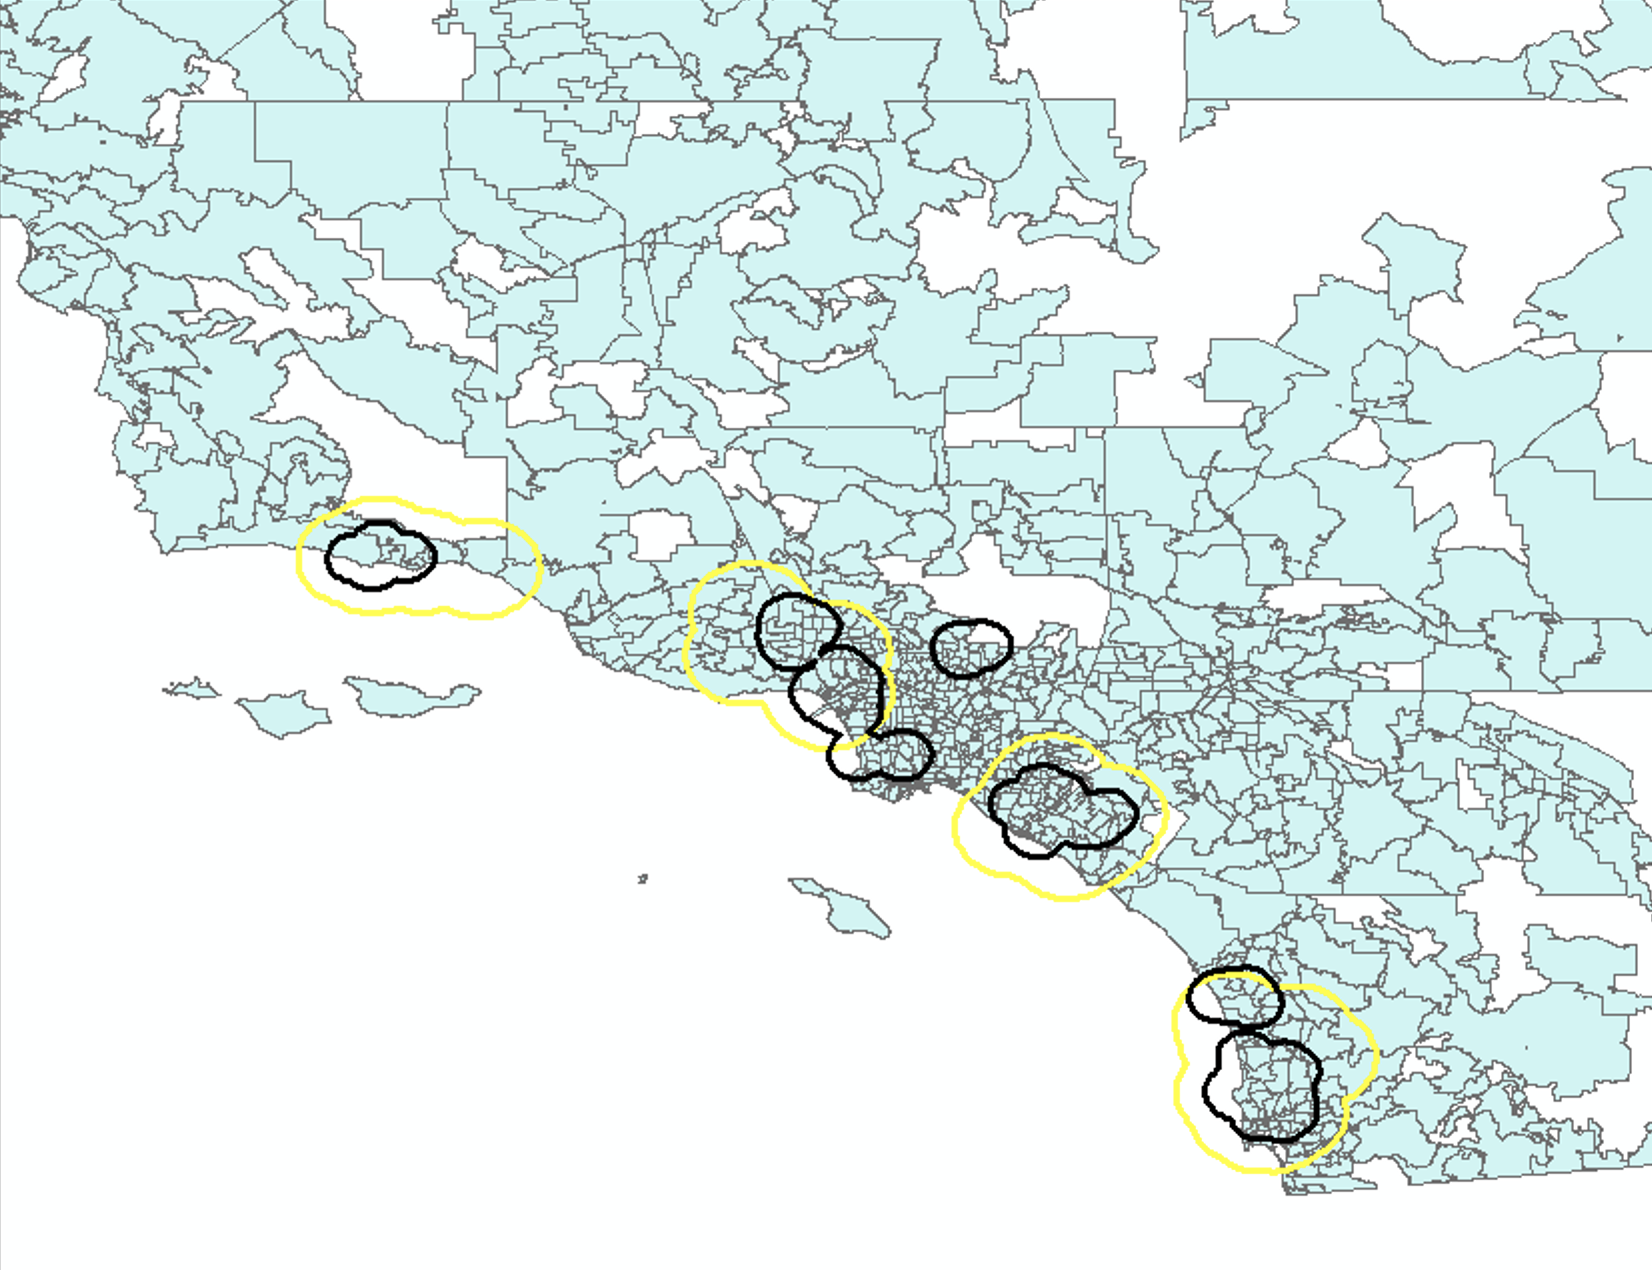
\includegraphics[width=9cm]{LA.png}
    \caption{5 and 10 Mile Clusters, San Diego, LA, and Santa Barbara}
    \label{fig:lab1}
\end{figure}
\begin{figure}[H]
    \centering
    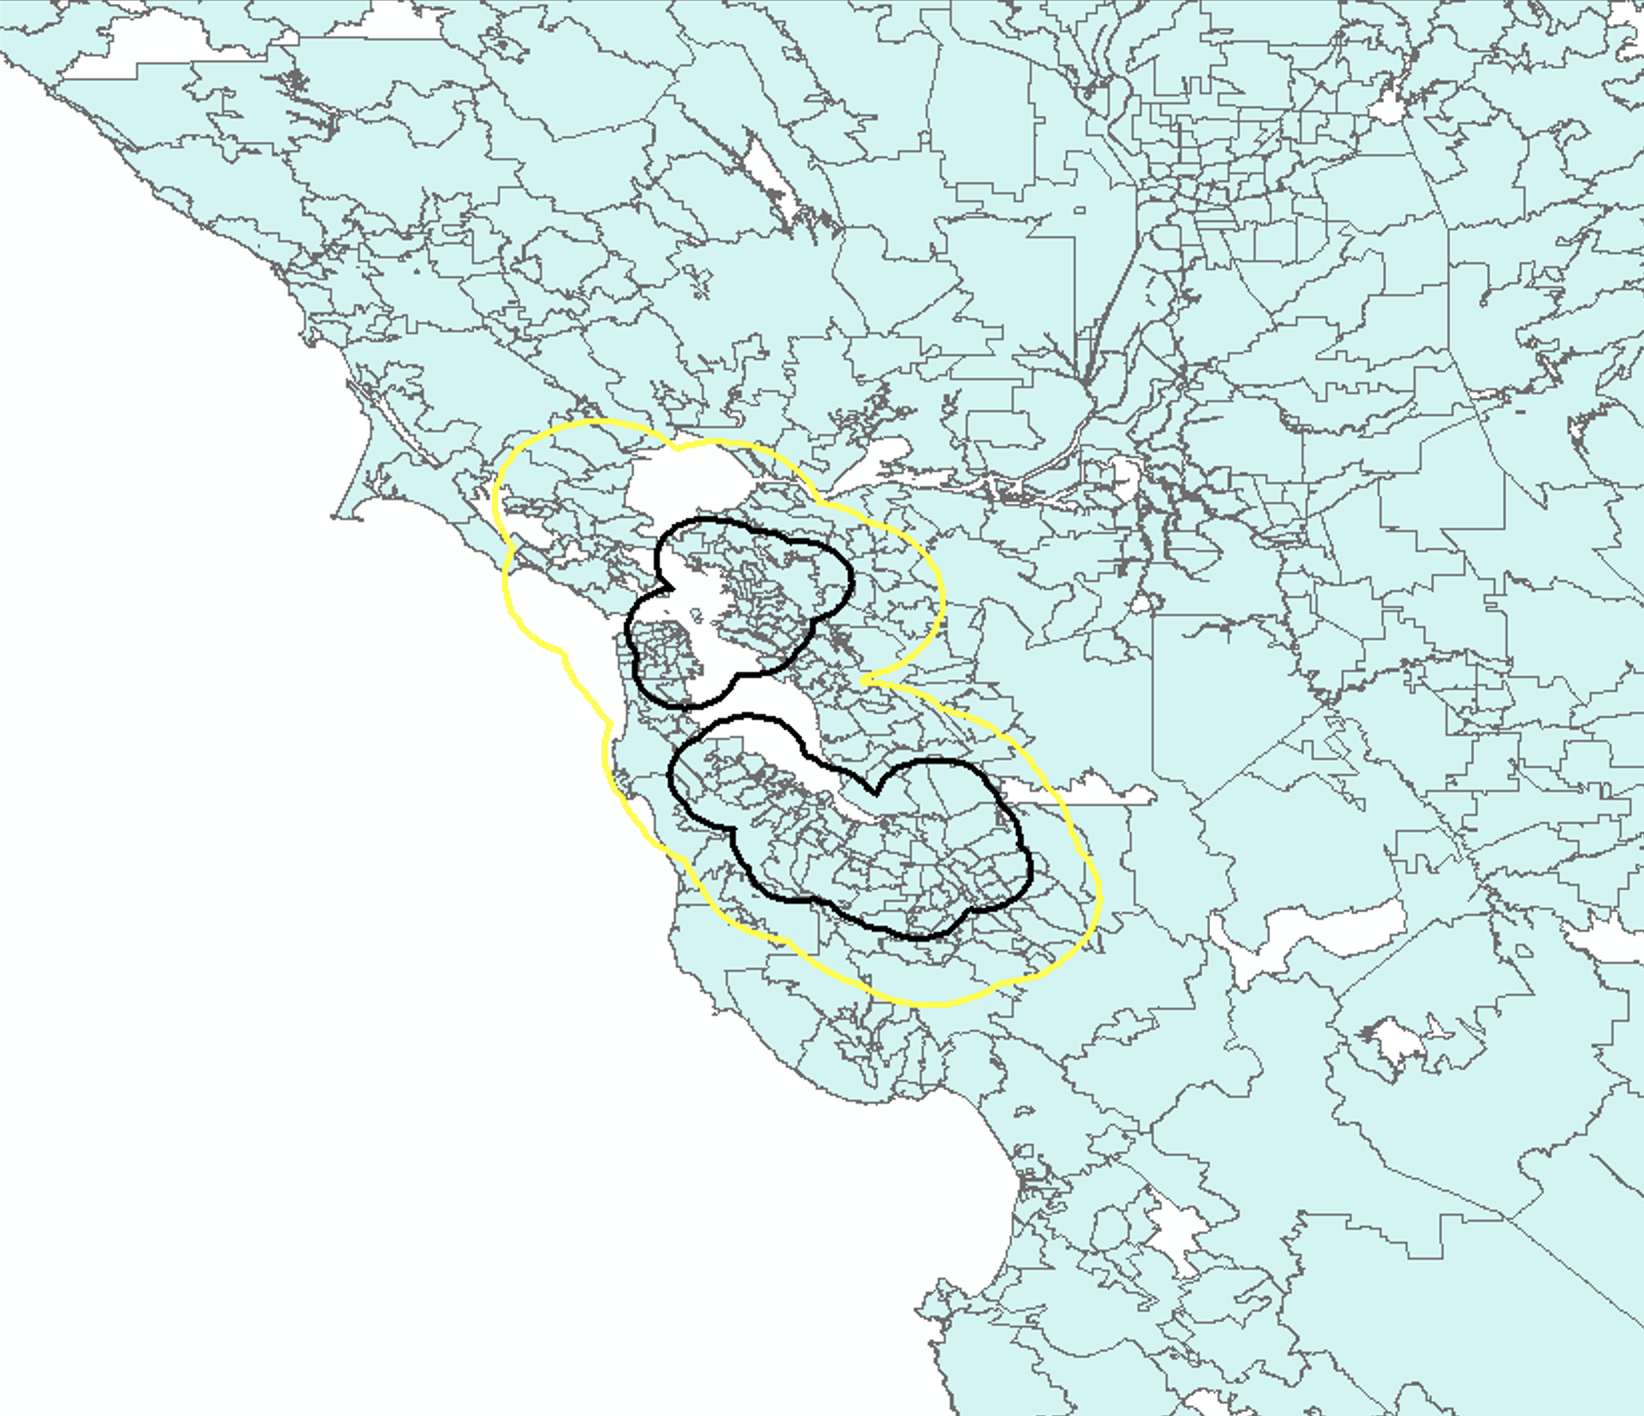
\includegraphics[width=9cm]{SF.png}
    \caption{5 and 10 mile clusters San Francisco}
    \label{fig:lab2}
\end{figure}
Figures 1 and 2 plot the locations of the clusters identified both at the five and ten mile spatial scales. As you can see the vast majority of the five mile clusters are held within the ten mile clusters. However, there are still pockets of independent five mile clusters such as in Northern Los Angeles. For the two ten mile clusters identified around Los Angeles, I think it is important to note that they are both on coastal areas away from the city center. In fact, all ten mile clusters identified in California reside on the coastline. This could largely be due to the fact that California's largest cities are all on the coast. Moreover, this serves to reinforce the use of these clusters as geographic boundaries for my knowledge spillover analysis since I am relying on the zip-code centroid of the \textbf{residential} address of inventors. If identified cluster locations significantly deviated from the largest population centers, clusters would serves as poor demarcations for the boundaries of localized knowledge spillovers since they wouldn't capture the patents that are actually being devised in the labs analyzed. 

\subsection{Research Field Clusters}
\begin{figure}[H]
    \centering
    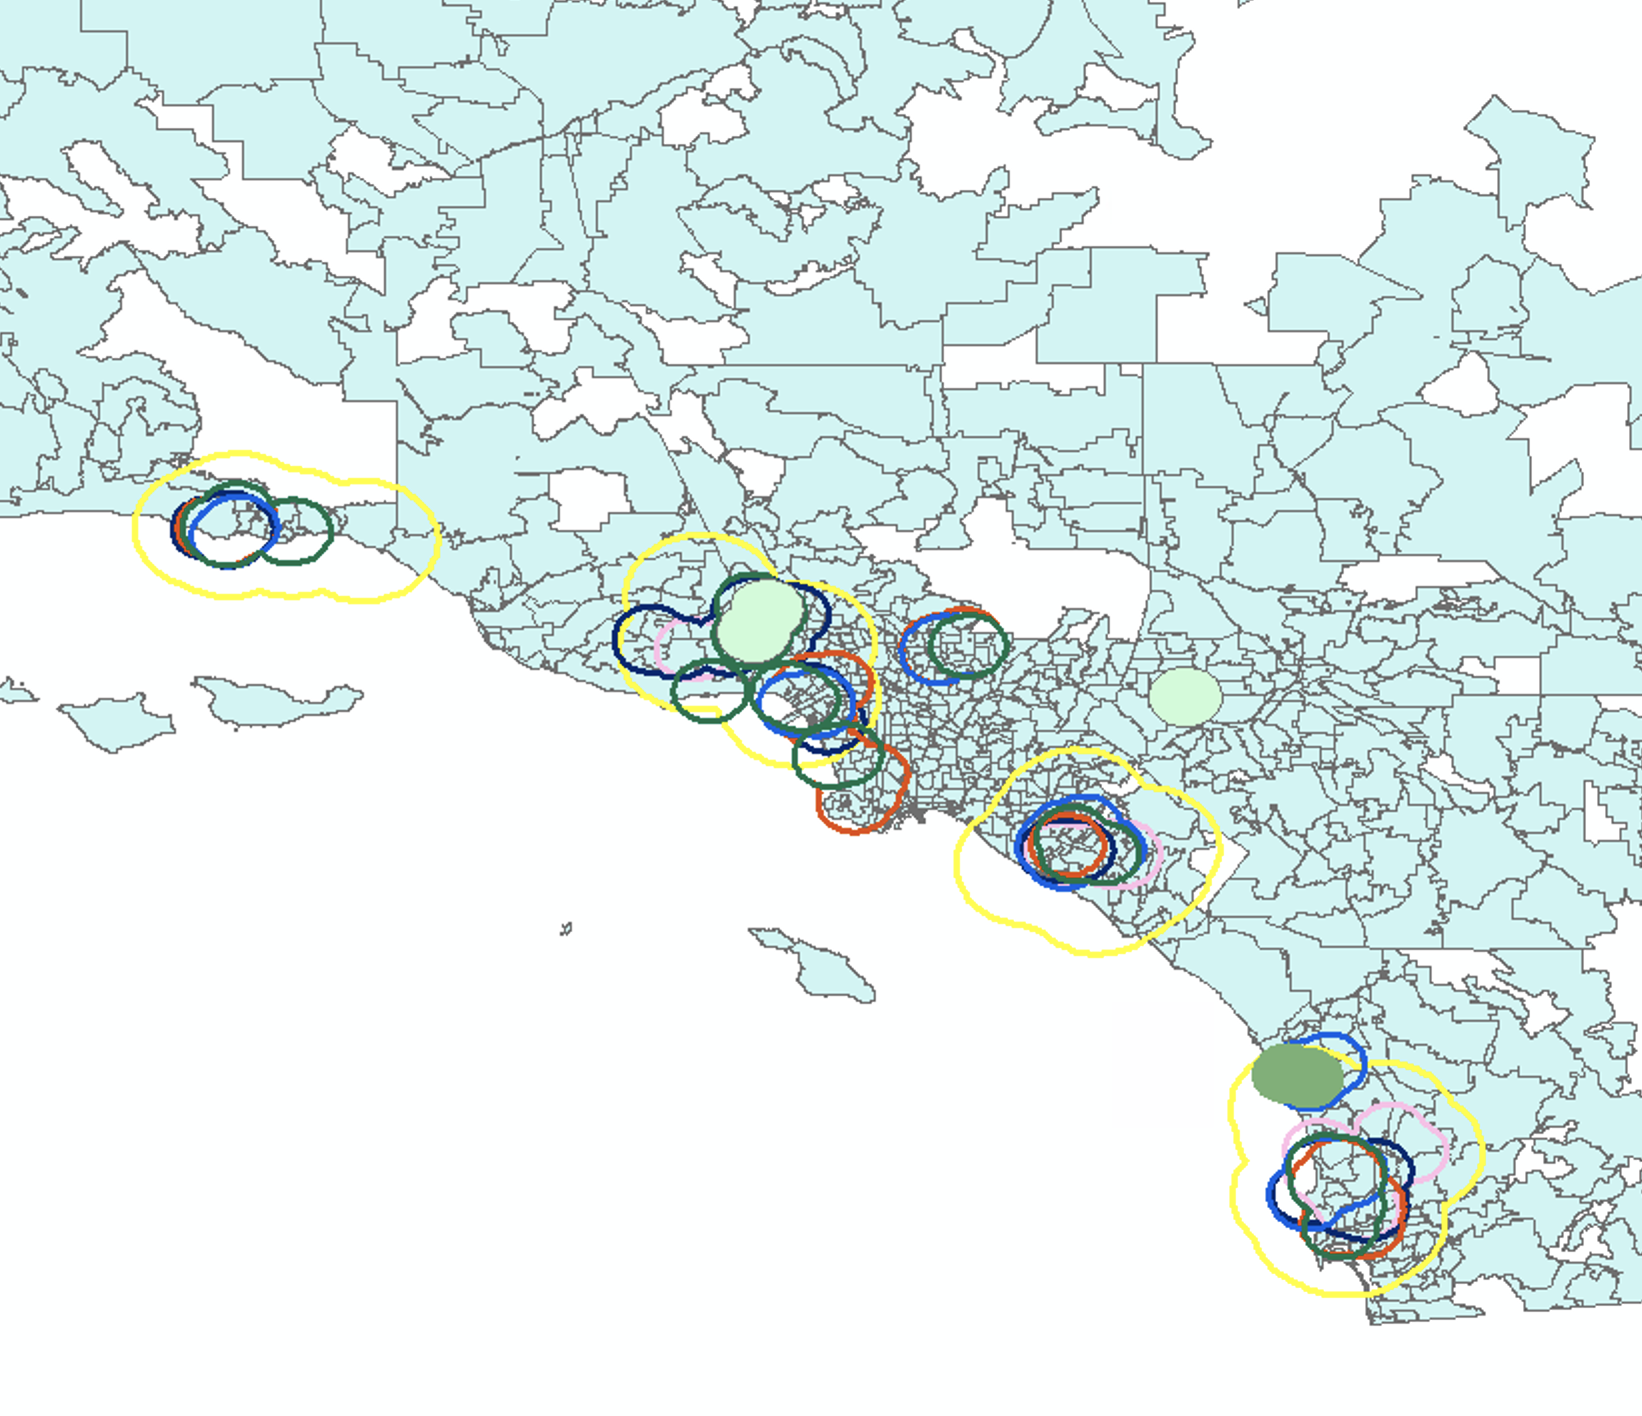
\includegraphics[width=9cm]{RLA.png}
    \caption{10 mile general clusters with select 5 Mile Research Field Clusters in SD LA and SB}
    \label{fig:lab3}
\end{figure}
\begin{figure}[H]
    \centering
    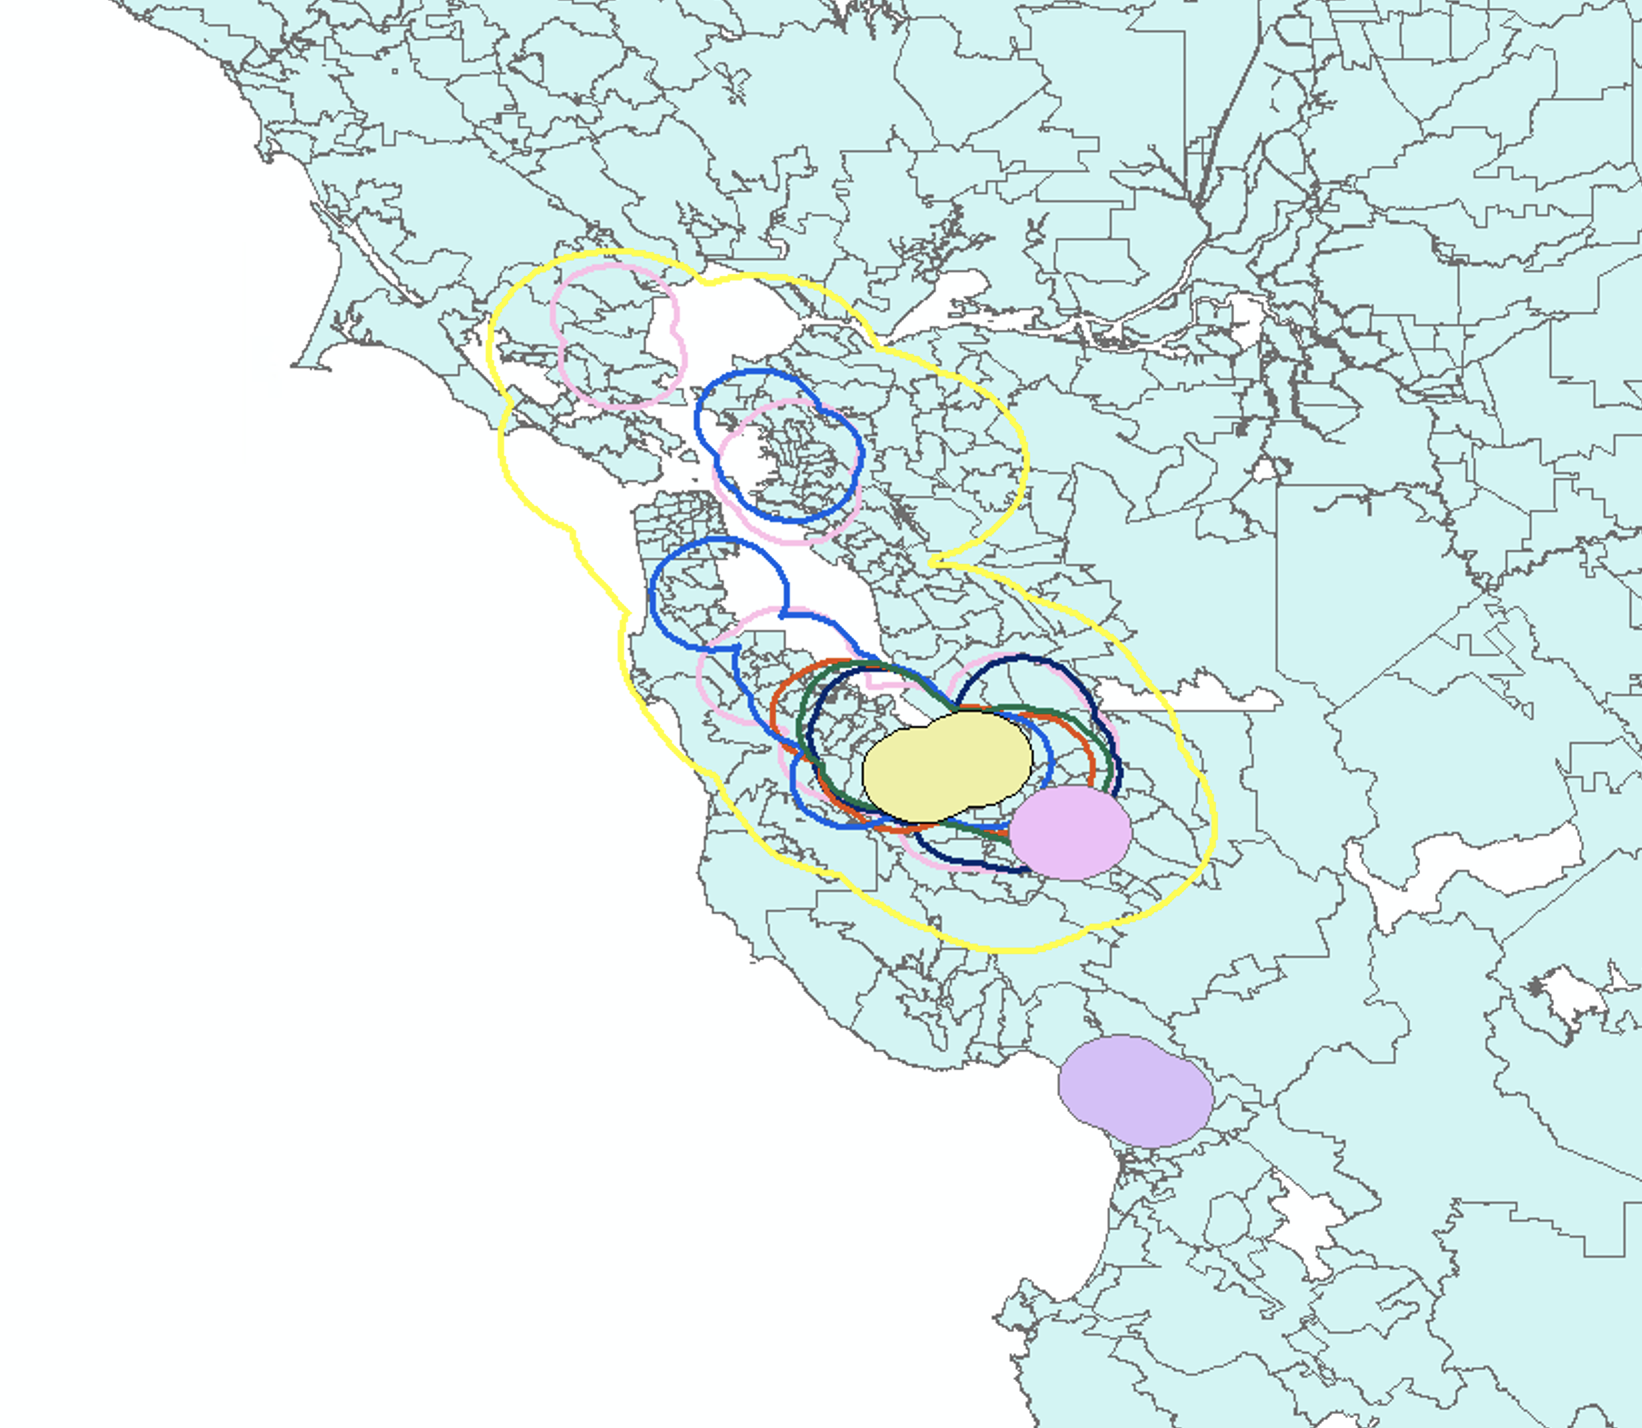
\includegraphics[width=9cm]{RSF.png}
    \caption{10 mile general clusters with select 5 mile research field clusters in SF}
    \label{fig:lab4}
\end{figure}
\par 
Figure 3 and 4 plot the 10 mile general clusters (large yellow outlines), the five mile clusters for the five research fields with the most labs\footnote{Full table with lab counts for each research field is in Table 8 in the appendix} in California (smaller multi-color outlines), and the five mile clusters for the five research fields with the fewest labs in California, above 30 (solid multi-color fill). From both figures it is apparent labs cluster intensely near similar labs. 
\par
Moreover, the significant amount of overlap between the clusters, both the ones of the largest research fields and the smallest indicate that there are still strong forces beyond being around the same firm driving the agglomeration of even the smallest areas of research. I take this high level of cluster diversity to indicate that there are particular agglomeration forces promoting heterogeneous clusters of labs. 
\par 
Furthermore, in the appendix I report the mean p-values for all labs within each research field that was analyzed. I find that in contrast to the general clusters, where clustering occurred most commonly at one and two miles, when analyzing clustering at the level of research field I find that clustering is most common at two, five, and ten mile spatial scales depending on research field. I take this result to suggest that there are geographic gaps between homogeneous labs which are occupied by heterogeneous labs. Or more simply, labs clusters do not necessarily focus around like labs but have a combination of both like and unlike labs, when considering research field. 
\par
As further evidence of the significance of heterogeneous lab agglomeration I report\footnote{Table 9 in appendix.} the proportions of labs from each research field which are inside one of the research field's one mile clusters and the proportion which are not in their research field's clusters. The average proportion of labs outside their research field's cluster is around 90\%\footnote{This is the average of reported proportions of labs outside their research field's one mile clusters in Table 9 in the appendix.} 

\subsection{General Knowledge Spillovers}
 
I report the results of the strength of knowledge spillovers within the five mile general clusters in table 3 below. In column \textbf{K}, I report the location differentials in the same cluster citation rate between my treatment group and my control group. Column \textbf{A} reports the number of originating patents considered for each cluster, column \textbf{B} reports the number of citing patents, column \textbf{C} reports the number of citing patents, column \textbf{B}, which were authored by an inventor living in the same cluster as the originating patents. Column \textbf{D} then reports the percentage of citing patents which come from the same cluster as the originating patents. Column \textbf{E} reports the number of treatment patents for each cluster and column \textbf{H} reports the number of controls. Columns \textbf{F} and \textbf{G} report the number of those patents in columns \textbf{E} and \textbf{H} which come from the same cluster as an originating patent. Columns \textbf{G} and \textbf{J} report the respective proportions for the treatment and control group. Finally, column \textbf{K} reports the total location differential which is just the amount of times which a treatment patent will cite a patent from the same cluster compared to the control.
\begin{table}[H]
\centering
\resizebox{\textwidth}{!}{%
\begin{tabular}{rllllllllllllll}
\hline
                     & Column           &      & A     & B      & C       & D      & E      & F        & G      & H      & I       & J      & K     &       \\ \hline
 & 5 Mile Clusters  & \# of & Originating & Citing & Same  & Percent & Treatment* & Same  & Percent & Control** & Same** & Percent & Differential & P-value \\
\multicolumn{1}{l}{} &                  & labs &       &        & Cluster & (C/B)  &        & Cluster* & (F/E)  &        & Cluster & (I/H)  & (G/J) &       \\ \cline{2-15} 
                     & San Diego\_S     & 144  & 1639  & 15731  & 608     & 0.0386 & 15728  & 608      & 0.0387 & 15728  & 206     & 0.0131 & 3     & 0.001 \\
                     & San Diego\_N     & 32   & 239   & 1545   & 42      & 0.0272 & 1544   & 42       & 0.0272 & 1544   & 8       & 0.0052 & 5.2   & 0.001 \\
                     & Los Angeles\_SE  & 150  & 741   & 6086   & 246     & 0.0404 & 6083   & 246      & 0.0404 & 6083   & 35      & 0.0058 & 7     & 0.001 \\
                     & Los Angeles\_W   & 209  & 1038  & 7151   & 232     & 0.0324 & 7151   & 232      & 0.0324 & 7151   & 42      & 0.0059 & 5.5   & 0.001 \\
                     & Los Angeles\_N   & 48   & 357   & 3216   & 155     & 0.0482 & 3213   & 155      & 0.0482 & 3213   & 7       & 0.0022 & 22.1  & 0.001 \\
                     & Santa Barbara    & 48   & 274   & 3141   & 128     & 0.0408 & 3141   & 128      & 0.0408 & 3141   & 6       & 0.0019 & 21.3  & 0.001 \\
 & San Francisco\_S & 427   & 7571        & 101431 & 12827 & 0.1265  & 101369     & 12816 & 0.1264  & 101369    & 5978   & 0.059   & 2.1          & 0.001   \\
                     & San Francisco\_N & 108  & 404   & 3872   & 69      & 0.0178 & 3870   & 69       & 0.0178 & 3870   & 11      & 0.0028 & 6.3   & 0.001 \\
                     & Total            & 1166 & 12263 & 142173 & 14307   & 0.1006 & 142099 & 14296    & 0.1006 & 142099 & 6293    & 0.0443 & 2.3   & 0     \\ \hline
\end{tabular}
}
\caption{}
\label{tab:3}
\end{table}
\par
Of particular note, in table 3, are the differentials for Santa Barbara and Los Angeles North, both demonstrate location differentials of more than 20. Meaning that for those two particular clusters the treatment group cited a patent within the same cluster 20 times more often than the control group did. However, both of these clusters are relatively small when considering the number of patents and labs contained within them. On average the strength of the knowledge spillovers identified within the five mile general clusters is a location differential of 2.3 as reported by the \textbf{"Total"} row and \textbf{K} column. As such, the strength of knowledge spillovers identified here are significantly smaller than those identified by Buzard et al. 


\begin{table}[H]
\centering
\resizebox{\textwidth}{!}{%
\begin{tabular}{rllllllllllllll}
\hline
  & Column          &      & A     & B      & C     & D      & E      & F     & G      & H      & I     & J      & K    & L     \\ \hline
0 &
  10 Mile &
  \# of &
  Originating &
  Citing &
  From Same &
  Percent &
  Treatment &
  From Same &
  Percent &
  Control &
  From Same &
  Percent &
  Differential &
  P-value \\
\multicolumn{1}{l}{} &
  Clusters &
  labs &
  Patents &
  Patents &
  Cluster &
  (C/B) &
  Patents* &
  Cluster* &
  (F/E) &
  Patents** &
  Cluster &
  (I/H) &
  (G/J) &
   \\ \hline
1 & San Diego       & 204  & 2186  & 19745  & 1049  & 0.0531 & 19741  & 1049  & 0.0531 & 19741  & 328   & 0.0166 & 3.2  & 0.001 \\
2 & Los Angeles\_SE & 186  & 1201  & 9951   & 461   & 0.0463 & 9945   & 461   & 0.0464 & 9945   & 88    & 0.0088 & 5.2  & 0.001 \\
3 & Los Angeles\_NW & 174  & 822   & 6150   & 177   & 0.0288 & 6150   & 177   & 0.0288 & 6150   & 30    & 0.0049 & 5.9  & 0.001 \\
4 & Santa Barbara   & 54   & 294   & 3298   & 129   & 0.0391 & 3298   & 129   & 0.0391 & 3298   & 7     & 0.0021 & 18.4 & 0.001 \\
5 &
  San Francisco &
  606 &
  10677 &
  137982 &
  23561 &
  0.1708 &
  137907 &
  23549 &
  0.1708 &
  137907 &
  11201 &
  0.0812 &
  2.1 &
  0.001 \\
6 & Total           & 1224 & 15180 & 177126 & 25377 & 0.1433 & 177041 & 25365 & 0.1433 & 177041 & 11654 & 0.0658 & 2.2  & 0     \\ \hline
\end{tabular}
}
\caption{}
\label{tab:4}
\end{table}

Table 4 above reports the results for the knowledge spillover analysis done using clusters with a ten mile radius. All columns are organized in the same way as in table 3. The results of note here are mainly in Santa Barbara. The location differential for the ten mile cluster in Santa Barbara is still incredibly high. However, it has gone down significantly from the amount reported for the 5 mile cluster in table 3. I take this as an indicator that the strength of knowledge spillovers attenuate with distance. However, the total strength of knowledge spillovers at the 10 mile cluster radius is almost exactly the same as that foe the 5 mile clusters. Moreover, the strong knowledge spillovers that appeared in Los Angeles North disappear and have little affect on the strength of knowledge spillovers in Los Angeles when considering 10 mile clusters. This suggests that the attenuation of knowledge spillovers is more complicated than suggested by Buzard et al.. My results suggest that the attenuation of knowledge spillovers has to do with both the distance at which they are observed and the quantity of patents being issued in the space observed. 
\begin{table}[H]
\centering
\resizebox{\textwidth}{!}{%
\begin{tabular}{rlrrrrrr}
\hline
                     & Cluster & \# of                        & Originating                 & Citing                      & Treatment                      & Control                        & Location                         \\
\multicolumn{1}{l}{} & Size    & \multicolumn{1}{l}{Clusters} & \multicolumn{1}{l}{Patents} & \multicolumn{1}{l}{Patents} & \multicolumn{1}{l}{Proportion} & \multicolumn{1}{l}{Proportion} & \multicolumn{1}{l}{Differential} \\ \hline
0                    & 5-Mile  & 8                            & 12263                       & 142173                      & 0.1006                         & 0.0443                         & 2.3                              \\
1                    & 10-Mile & 5                            & 15180                       & 177126                      & 0.1433                         & 0.0658                         & 2.2                              \\ \hline
\end{tabular}%
}
\caption{}
\label{tab:5}
\end{table}
Table 5 aggregates the results from tables 3 and 4 and presents the total number of originating and citing patents at each spatial scale. The \textbf{"Treatment Proportion"} and \textbf{"Control Proportion"} columns give the proportion of treatment and control patents which were attributed to an inventor living within the same cluster as the originating patent at each spatial scale. 
Interestingly, as mentioned earlier, the location differentials are relatively constant when expanding the scale of observation from five to ten miles. The lack of attenuation in the strength of knowledge spillovers from one spatial scale to another indicates to me that by increasing the geographic area of analysis with more labs we may have reached a lower bound to the strength of knowledge spillovers within geographic boundaries. This is particularly reinforced by the fact that the location differentials I observe are comparable to those observed by JTH\footnote{In their seminal 1993 paper on knowledge spillovers, JTH find an average location differential at the state level of 2. Similar to my location differential at both five and ten miles.} at the state level, an even larger geographic boundary from what I have analyzed.  

\subsection{Knowledge Spillovers by Technology Categories}
In an attempt to further understand the driving forces behind lab agglomeration and the knowledge spillovers that become evident from it, I group the labs from the 1998 Dart and the patents from the citation matching into six technology categories\footnote{a table containing the allocation of research fields and patent codes into the six technology categories in the appendix under table 10} based on the demarcations done by HJT. I analyze the resulting set of labs and patents as described in section 3.6.
\begin{table}[H]
\tiny
\centering
\begin{tabular}{rlrrrrrrrr}
\multicolumn{1}{l}{} &       & A           & B           & C        & D        & E        & F        & G        & H        \\ \hline
 & Categories & prop\_5 & prop\_10 & hhi\_5 & hhi\_10 & 5 mile prop\_in & 5 mile prop\_out & 10 mile prop\_in & 10 mile prop\_out \\ \hline
0                    & chem  & 0.0010377   & 0.000104791 & 0.599048 & 0.563098 & 0.112375 & 0.887625 & 0.157048 & 0.842952 \\
1                    & comp  & 0.000689151 & 0.000203054 & 0.572913 & 0.541661 & 0.384388 & 0.615612 & 0.472619 & 0.527381 \\
2                    & drug  & 0.000746244 & 0.000273522 & 0.518237 & 0.536717 & 0.35373  & 0.64627  & 0.38485  & 0.61515  \\
3                    & elec  & 6.12466e-05 & 7.95909e-05 & 0.561235 & 0.587815 & 0.201183 & 0.798817 & 0.280382 & 0.719618 \\
4                    & mech  & 8.79454e-05 & 1.65311e-05 & 0.194324 & 0.185938 & 0.169036 & 0.830964 & 0.195652 & 0.804348 \\
5                    & other & 0.000257537 & 2.72713e-05 & 0.215238 & 0.174072 & 0.118359 & 0.881641 & 0.162128 & 0.837872 \\ \hline
\end{tabular}
\caption{}
\label{tab:6}
\end{table}
The results of my analysis are presented above in table 6. Columns \textbf{A} and \textbf{B} report the proportion of citing patents which cite a patent from the same cluster on a per lab basis. Essentially, this is the proportion of citations coming from the same cluster for each technology category adjusted for the amount of labs in each technology category. I take these results as indicators of the technological categories which are most driving the knowledge spillovers within the clusters at each scale. As is clear by the results in both columns \textbf{A} and \textbf{B}, innovation in chemicals technology is driving the knowledge spillovers I identify at five and ten miles. More importantly though, the two most significant contributors to knowledge spillovers, chemical technology and computational technology, both have drastically different proportions of labs within their technical clusters vs outside of those clusters as shown in columns
\textbf{E, F, G} and \textbf{H}. I take this to indicate that different technology categories take advantage of different types of spillovers. Seeing as research into chemical technology gas more than 80\% of its labs outside of technical clusters I would claim that such research primarily takes advantage of heterogeneous Jacobs style knowledge spillovers. On the other hand, research into computational technology has only around 60\% of its labs outside of a technical cluster, indicating, such research may benefit more from the homogeneous MAR style spillovers. 

\section{Conclusion}
By this point it is obvious that R\&D labs, in the state of California, cluster more significantly than economic activity would suggest. However, the drivers of this agglomeration are still unknown. My research paints a picture of some of the possible driving forces behind this agglomeration and the types of agglomeration they lead to. Moreover, I am able to evaluate which forms of research are currently leveraging the knowledge spillover advantages, gained from lab agglomeration, the most. I note that chemicals research is the principal driver of knowledge spillovers at both the five and ten mile scale. However, seeing as the next strongest driver is clustered in a different form, it is unclear what types of clustering, heterogeneous or homogeneous, take the most advantage of these knowledge spillovers. Overall though I am able to paint a picture of the lab agglomeration present within California. I demonstrate both the heterogeneous and homogeneous agglomeration that is present and based on the spatial scales it occurs I predict that labs agglomerate more heterogenously than homogeneously. 

\newpage
\section{References}    
\par 
Buzard, Kristy, Carlino, Gerald A., Hunt, Robert M., Carr, Jake K., Smith, Tony E., 2017.Theagglomeration of American RD labs. J. Urban Econ. 101, 14–26.
\par 
K. Buzard, G.A. Carlino, R.M. Hunt, J.K. Carr, and T.E. Smith. Localized knowledge spillovers:Evidence from the agglomeration of american rd labs and patent data, 2017.
\par 
D.B. Audrescht and M.P. Feldman.  Rd spillovers and the the geography of innovation andproduction, 1996
\par 
Directory of American Research and Technology, 23rd Ed. New York: R.R. Bowker (1999)
\par
G. Ellison and E.L. Glaser.   Geographic concentration in u.s.   manufacturing industries:  adartboard approach, 1997.
\par
Getis, Arthur. “Interaction Modeling Using Second-Order Analysis,” Environment and Planning,16 (1984), pp. 173–83.
\par
Edward Glaeser, Hedi Kallal, Jose Scheinkman, and Andrei Shleifer, who coined the term
\par 
Hall, Bronwyn H.; Jaffe, Adam B. and Trajten- berg, Manuel. ”The NBER Patent Citation DataFile: Lessons, Insights and Methodolog- ical Tools.” National Bureau of Economic Research, Inc.
\par
The city. The economy of the cities. By Jane Jacobs. Random House, 201 East 50th Street, NewYork 10022, 1969. 268 pp
\par
Jaffe, Adam B.; Trajtenberg, Manuel and Henderson, Rebecca. ”Geographic Localiza- tion ofKnowledge Spillovers as Evidenced by Patent Citations.” Quarterly Journal of Economics, 1993,108(3), pp. 577-98
\par
Png, Ivan, 2019, ”U.S. RD 1975-1998: A New Dataset”, https://doi.org/10.7910/DVN/7QYFFB,Harvard Dataverse, V2, UNF:6:n3RVowZQLU7cY6PkW77z9g== [fileUNF]
\par
Ripley, Brian D. “The Second-Order Analysis of Stationary Point Patterns,” Journal of AppliedProbability, 13 (1976), pp. 255–66
\par
S. Rosenthal and W.C. Strange. The determinants of agglomeration, 2001.
\par
Steven Manson, Jonathan Schroeder, David Van Riper, Tracy Kugler, and Steven Ruggles. IPUMSNational Historical Geographic Information System:  Version 15.0 [dataset].  Minneapolis, MN:IPUMS. 2020. http://doi.org/10.18128/D050.V15.
%remember to use \citep{} for citation



\newpage
\section{Appendix}
\begin{table}[H]
\centering
\resizebox{\textwidth}{!}{%
\begin{tabular}{rlrrrrrrr}
\hline
 & field & P\_025\_mean & P\_05\_mean & P\_075\_mean & P\_1\_mean & P\_2\_mean & P\_5\_mean & P\_10\_mean \\ \hline
0  & ELEN & 0.283882 & 0.226248 & 0.202212 & 0.203923 & 0.197156 & 0.258926 & 0.310589 \\
1  & COMP & 0.35483  & 0.265651 & 0.21929  & 0.195102 & 0.186463 & 0.212695 & 0.228486 \\
2  & PHYS & 0.286995 & 0.261011 & 0.247768 & 0.250527 & 0.224445 & 0.323539 & 0.335129 \\
3  & ENGI & 0.477512 & 0.416059 & 0.363605 & 0.321939 & 0.278887 & 0.299147 & 0.303873 \\
4  & MEDI & 0.266698 & 0.235317 & 0.206433 & 0.194243 & 0.190186 & 0.225507 & 0.260817 \\
5  & CHEM & 0.415237 & 0.393045 & 0.347401 & 0.327045 & 0.302689 & 0.357805 & 0.373503 \\
6  & COMM & 0.367462 & 0.316578 & 0.286565 & 0.26998  & 0.242744 & 0.256532 & 0.250468 \\
7  & INDU & 0.546542 & 0.485215 & 0.477102 & 0.452916 & 0.363065 & 0.416971 & 0.442225 \\
8  & ELEC & 0.369318 & 0.348096 & 0.319619 & 0.32069  & 0.280067 & 0.32282  & 0.348778 \\
9  & AERO & 0.468838 & 0.438885 & 0.423316 & 0.405855 & 0.344996 & 0.348744 & 0.322756 \\
10 & ENVI & 0.340677 & 0.332301 & 0.29555  & 0.285437 & 0.259585 & 0.319245 & 0.289594 \\
11 & META & 0.432214 & 0.41106  & 0.404185 & 0.406113 & 0.337964 & 0.370167 & 0.384649 \\
12 & MANA & 0.454135 & 0.366961 & 0.352239 & 0.340858 & 0.283252 & 0.221232 & 0.243781 \\
13 & SECU & 0.429838 & 0.420291 & 0.405662 & 0.36525  & 0.330662 & 0.336392 & 0.347358 \\
14 & PLAS & 0.358398 & 0.366797 & 0.363361 & 0.355098 & 0.348707 & 0.328135 & 0.401406 \\
15 & CONS & 0.729397 & 0.661809 & 0.586504 & 0.543061 & 0.452214 & 0.368901 & 0.299916 \\
16 & BIOL & 0.486246 & 0.474    & 0.438426 & 0.395672 & 0.354803 & 0.339795 & 0.363877 \\
17 & FOOD & 0.387367 & 0.358467 & 0.35025  & 0.332117 & 0.324292 & 0.319842 & 0.398033 \\
18 & PHAR & 0.503577 & 0.421721 & 0.398558 & 0.395865 & 0.385462 & 0.331317 & 0.308096 \\
19 & FUEL & 0.438149 & 0.43     & 0.378894 & 0.359681 & 0.290383 & 0.334734 & 0.401819 \\
20 & CNST & 0.604188 & 0.596787 & 0.59025  & 0.592525 & 0.502637 & 0.44705  & 0.4083   \\
21 & AUTO & 0.62912  & 0.593587 & 0.50932  & 0.474987 & 0.361347 & 0.375547 & 0.36632  \\
22 & SOCI & 0.223274 & 0.214055 & 0.220562 & 0.228726 & 0.24737  & 0.215068 & 0.259178 \\
23 & AGRI & 0.531076 & 0.531803 & 0.53247  & 0.533439 & 0.514333 & 0.37147  & 0.487621 \\
24 & AVIA & 0.565758 & 0.551806 & 0.555742 & 0.544226 & 0.480226 & 0.451823 & 0.462    \\
25 & TRAN & 0.668316 & 0.635298 & 0.604035 & 0.57486  & 0.456544 & 0.422123 & 0.36693  \\
26 & EART & 0.399396 & 0.329189 & 0.332604 & 0.318887 & 0.330491 & 0.309755 & 0.376849 \\
27 & NUCL & 0.479938 & 0.480479 & 0.481583 & 0.482583 & 0.355979 & 0.318    & 0.235458 \\
28 & PAPE & 0.815148 & 0.741778 & 0.635222 & 0.637111 & 0.60963  & 0.538444 & 0.396889 \\
29 & TEXT & 0.750667 & 0.751917 & 0.753917 & 0.756    & 0.692875 & 0.494125 & 0.544833 \\
30 & CERA & 0.778    & 0.778444 & 0.779444 & 0.780667 & 0.786889 & 0.663167 & 0.686389 \\
31 & EDUC & 1        & 0.847308 & 0.848154 & 0.849231 & 0.699923 & 0.582923 & 0.477846 \\
32 & RECR & 1        & 1        & 1        & 1        & 1        & 1        & 0.678375 \\ \hline
\end{tabular}
}
\caption{}
\label{tab:7}
\end{table}

\begin{table}[H]
\scriptsize
\centering
\begin{tabular}{ll}
\hline
field & count \\ \hline
ELEN  & 661   \\
COMP  & 588   \\
PHYS  & 559   \\
ENGI  & 443   \\
MEDI  & 403   \\
CHEM  & 353   \\
COMM  & 300   \\
INDU  & 274   \\
ELEC  & 239   \\
AERO  & 235   \\
ENVI  & 229   \\
META  & 168   \\
MANA  & 156   \\
SECU  & 149   \\
PLAS  & 133   \\
CONS  & 130   \\
BIOL  & 121   \\
FOOD  & 120   \\
PHAR  & 104   \\
FUEL  & 94    \\
CNST  & 80    \\
AUTO  & 76    \\
SOCI  & 75    \\
AGRI  & 66    \\
AVIA  & 63    \\
TRAN  & 58    \\
EART  & 53    \\
NUCL  & 48    \\
PAPE  & 27    \\
TEXT  & 24    \\
CERA  & 18    \\
EDUC  & 15    \\
RECR  & 8     \\
TAXO  & 1     \\ \hline
\end{tabular}
\caption{}
\label{tab:8}
\end{table}

\begin{table}[tbp]
\scriptsize
\centering
\begin{tabular}{rlrr}
\hline
   & field & prop\_in  & prop\_out \\ \hline
0  & ELEN  & 0.335855  & 0.664145  \\
1  & COMP  & 0.438776  & 0.561224  \\
2  & PHYS  & 0.286225  & 0.713775  \\
3  & ENGI  & 0.390519  & 0.609481  \\
4  & MEDI  & 0.384615  & 0.615385  \\
5  & CHEM  & 0.189802  & 0.810198  \\
6  & COMM  & 0.33      & 0.67      \\
7  & INDU  & 0.160584  & 0.839416  \\
8  & ELEC  & 0.246862  & 0.753138  \\
9  & AERO  & 0.357447  & 0.642553  \\
10 & ENVI  & 0.144105  & 0.855895  \\
11 & META  & 0.047619  & 0.952381  \\
12 & MANA  & 0.307692  & 0.692308  \\
13 & SECU  & 0.228188  & 0.771812  \\
14 & PLAS  & 0.0977444 & 0.902256  \\
15 & CONS  & 0.138462  & 0.861538  \\
16 & BIOL  & 0.272727  & 0.727273  \\
17 & FOOD  & 0.075     & 0.925     \\
18 & PHAR  & 0.403846  & 0.596154  \\
19 & FUEL  & 0.117021  & 0.882979  \\
20 & CNST  & 0.0875    & 0.9125    \\
21 & AUTO  & 0.118421  & 0.881579  \\
22 & SOCI  & 0.226667  & 0.773333  \\
23 & AGRI  & 0.030303  & 0.969697  \\
24 & AVIA  & 0.111111  & 0.888889  \\
25 & TRAN  & 0.12069   & 0.87931   \\
26 & EART  & 0.0943396 & 0.90566   \\
27 & NUCL  & 0.0208333 & 0.979167  \\
28 & PAPE  & 0         & 1         \\
29 & TEXT  & 0         & 1         \\
30 & CERA  & 0         & 1         \\
31 & EDUC  & 0         & 1         \\
32 & RECR  & 0         & 1         \\
33 & TAXO  & 0         & 1         \\ \hline
\end{tabular}
\caption{}
\label{tab:9}
\end{table}

\begin{table}[H]
\tiny
\centering
\begin{tabular}{lll}
\hline
Technological Category &
  Research Fields &
  Patent Codes \\ \hline
\multicolumn{1}{l|}{Chemical} &
  \multicolumn{1}{l|}{CHEM , FUEL,  AGRI} &
  \begin{tabular}[c]{@{}l@{}}8, 19, 71, 127, 442, 504, 106, 118, 401, 427, 48, 55, 95, 96, \\ 534, 536, 540, 544, 546, 548, 549, 552, 554, 556, 558, 560,\\ 562, 564, 568, 570, 520, 521, 522, 523, 524, 525,\\ 526, 527, 528, 530,  23, 34,  44, 102, 117, 149, 156,\\ 159, 162, 196, 201, 202, 203, 204, 205, 208, 210, 216, 222,\\ 252, 260, 261, 349, 366, 416,\\ 422, 423, 430, 436, 494, 501,502, 510, 512, 516, 518, 585,\\ 588\end{tabular} \\ \hline
\multicolumn{1}{l|}{\begin{tabular}[c]{@{}l@{}}Computers \&\\ Communications\end{tabular}} &
  \multicolumn{1}{l|}{COMP, COMM} &
  \begin{tabular}[c]{@{}l@{}}178, 333, 340, 342, 343, 358,\\ 367, 370, 375, 379, 385, 455, 341, 380, 382, 395, 700, 701,\\ 702, 704, 705, 706, 707, 708,709, 710, 712, 713, 714, 345, \\ 347, 360, 365, 369, 711\end{tabular} \\ \hline
\multicolumn{1}{l|}{Drugs \& Medical} &
  \multicolumn{1}{l|}{MEDI, BIOL, PHAR} &
  \begin{tabular}[c]{@{}l@{}}424, 514,128, 600, 601, 602, 604, \\ 606, 607, 435, 800, 351, 433, 623\end{tabular} \\ \hline
\multicolumn{1}{l|}{Electrical and Electronic} &
  \multicolumn{1}{l|}{ELEN, ELEC, NUCL} &
  \begin{tabular}[c]{@{}l@{}}174, 200, 327, 329, 330, 331,\\ 332, 334, 335, 336, 337, 338, 392, 439, 313, 314, 315, 362, \\ 372, 445, 73, 324, 356, 374, 73, 324, 356, 374, 73, 324, \\ 356, 374, 257, 326, 438, 505, 191, 218, 219, 307, 346, 348,\\ 377, 381, 386\end{tabular} \\ \hline
\multicolumn{1}{l|}{Mechanical} &
  \multicolumn{1}{l|}{\begin{tabular}[c]{@{}l@{}}META, PLAS, TRAN, \\ PAPE, ENGI, INDU, \\ PHYS, AUTO, AVIA, AERO\end{tabular}} &
  \begin{tabular}[c]{@{}l@{}}65, 82, 83, 125, 141, 142, 144,\\ 173, 209, 221, 225, 226, 234, 241, 242, 264, 271, 407, 408,\\ 409, 414, 425, 451, 493, 29, 72, 75, 76, 140, 147, 148,\\ 163, 164, 228, 266, 270, 413, 419, 420, 91, 92, 123, 185, 188, 192, 251,\\ 303, 415, 417, 418, 464, 474, 475, 476, 477, 352, 353, 355, 359, \\ 396, 399, 104, 105, 114, 152, 180, 187, 213, 238, 244, 246, 258, 280,\\ 293, 295, 296, 298, 301, 305, 410, 440, 7, 16, 42, 49, 51, 74, 81, 86, 89,\\ 100, 124, 157, 184, 193, 194, 198, 212, 227, 235, 239, 254,\\ 267, 291, 294, 384, 400, 402, 406, 411, 453, 454, 470, 482,\\ 483, 492, 508\end{tabular} \\ \hline
\multicolumn{1}{l|}{Others} &
  \multicolumn{1}{l|}{\begin{tabular}[c]{@{}l@{}}ENVI, MANA, FOOD,\\  SOCI, EART, EDUC, RECR,\\  TAXO, CONS, CNST, SECU\end{tabular}} &
  \begin{tabular}[c]{@{}l@{}}{[}43, 47, 56, 99, 111, 119, 131,\\ 426, 449, 452, 460, 273, 446, 463, 472, 473, 2, 12, 24, 26, \\ 28, 36, 38, 57, 66, 68, 69, 79, 87, 112, 139, 223,\\ 450, 37, 166, 171, 172, 175, 299, 405, 507,  4, 5, 30, 70, 132, 182, 211, 256,\\ 297, 312, 110, 122, 126, 165, 237, 373, 431, 432, 138, 277, 285, 403, 53, \\ 206, 215, 217, 220, 224, 229, 232, 383, 1, 14, 15, 27, 33, \\ 40, 52, 54, 59, 62, 63, 84, 101, 108, 109, 116,\\ 134, 135, 137, 150, 160, 168, 169, 177, 181, 186, 190, 199,\\ 231, 236, 245, 248, 249, 269, 276, 278, 279, 281, 283, 289,\\ 292, 300, 368, 404, 412, 428,\\ 434, 441, 462, 503\end{tabular} \\ \hline
 &
   &
  
\end{tabular}
\caption{}
\label{tab:10}
\end{table}

\begin{table}[H]
\scriptsize
\centering
\begin{tabular}{ll}
field & field\_name                    \\
ELEN  & ELECTRONICS                    \\
COMP  & COMPUTER                       \\
PHYS  & PHYSICS RESEARCH               \\
ENGI  & ENGINEERING                    \\
MEDI  & MEDICAL SCIENCES               \\
CHEM  & CHEMICALS RESEARCH             \\
COMM  & COMMUNICATIONS                 \\
INDU  & INDUSTRIAL PRODUCTS            \\
ELEC  & ELECTRIC AND POWER             \\
AERO  & AEROSPACE                      \\
ENVI  & ENVIRONMENTAL                  \\
META  & METALS AND METALLURGY          \\
MANA  & MANAGEMENT SCIENCES            \\
SECU  & SECURITY                       \\
PLAS  & PLASTICS                       \\
CONS  & CONSUMER PRODUCTS              \\
BIOL  & BIOLOGICAL RESEARCH            \\
FOOD  & FOOD                           \\
PHAR  & PHARMACEUTICS                  \\
FUEL  & FUELS                          \\
CNST  & CONSTRUCTION                   \\
AUTO  & AUTOMOTIVE                     \\
SOCI  & SOCIAL AND BEHAVIORAL SCIENCES \\
AGRI  & AGRICULTURE                    \\
AVIA  & AVIATION                       \\
TRAN  & TRANSPORTATION                 \\
EART  & EARTH SCIENCES                 \\
NUCL  & NUCLEAR RESEARCH               \\
PAPE  & PAPER AND WOOD                 \\
TEXT  & TEXTILE AND CLOTHING           \\
CERA  & CERAMICS                       \\
EDUC  & EDUCATIONAL                    \\
RECR  & RECREATION                     \\
TAXO  & TAXONOMIC STUDIES             
\end{tabular}
\caption{}
\label{tab:11}
\end{table}
\end{document}


\renewcommand{\arraystretch}{.75} % Default value: 1
\begin{tabular}{rrrr}
\hline
   Clust Radius &   Mean P Val &       HHI \\
\hline
   &       0.25 &   0.0050495  & 0.0689615 \\
   &       0.5  &   0.00963166 & 0.0698456 \\
   &       0.75 &   0.0100854  & 0.067957  \\
   &       1    &   0.0102258  & 0.0672329 \\
   &       2    &   0.0136941  & 0.0634257 \\
   &       5    &   0.0918774  & 0.0618392 \\
   &       10    &   0.107445   & 0.0636253 \\
\hline
\end{tabular}